\documentclass[aspectratio=169]{beamer}
\usepackage[utf8]{inputenc}
%\usepackage[width=160,height=90]{geometry}
\usepackage{graphicx}
\usepackage{multicol}

\renewcommand{\sfdefault}{phv}

\usetheme{Montpellier}

\definecolor{adngreen}{RGB}{0,167,127}
\setbeamercolor{title}{fg=white}

\setbeamercolor{frametitle}{fg=white}
\setbeamercolor{structure}{bg=adngreen,fg=adngreen}
\setbeamercolor{subsection in sidebar}{fg=white}





\title{\textbf{Lightning Talk} \\Indirect Direct Object Reference}
\author{Timo Bonomelli, Patrick Günthard}



\begin{document}

\frame{\titlepage}

\begin{frame}
  \frametitle{Table of Contents}
  \tableofcontents
\end{frame}
\section{Vulnerability}

\begin{frame}
  \frametitle{What is \textit{Insecure Direct Object References}}
  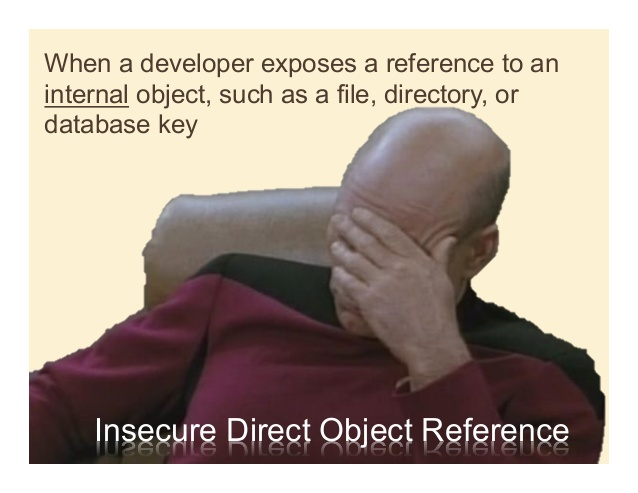
\includegraphics[width=8cm]{meme}
\end{frame}

\subsection{Threats}

\begin{frame}
  \frametitle{Threats}
  \begin{itemize}
  \item \textbf{Threat Agents:} Any user who has only partial access to certain type of system data
  \item \textbf{Attacker’s Approach:} Attacker, an authorized system user, simply changes a parameter value that directly refers to a system object to another object the user isn’t authorized to use
  \item \textbf{Security Weakness:} Applications don’t always verify the user is authorized for target objects
  \end{itemize}
\end{frame}

\subsection{Example}

\begin{frame}[fragile]
  \label{examplecode}
  \frametitle{Example: Code}
  \textit{Example Website:}\\\tiny
\dots
\begin{verbatim}
$conn = new mysqli(...);
$conn->query("UPDATE tbl_user SET password = '".$_GET['pw']."' WHERE username = '".$_GET['user']."';)
\end{verbatim}
\dots
\normalsize
\end{frame}


\begin{frame}
  \frametitle{Example: Attack}
  \begin{multicols}{2}
   \LARGE{Normal behavior}\\\normalsize Example URL: \small\texttt{http://somesite.net/change password?user=\textit{myuser}}\\
   \normalsize{Result:}\\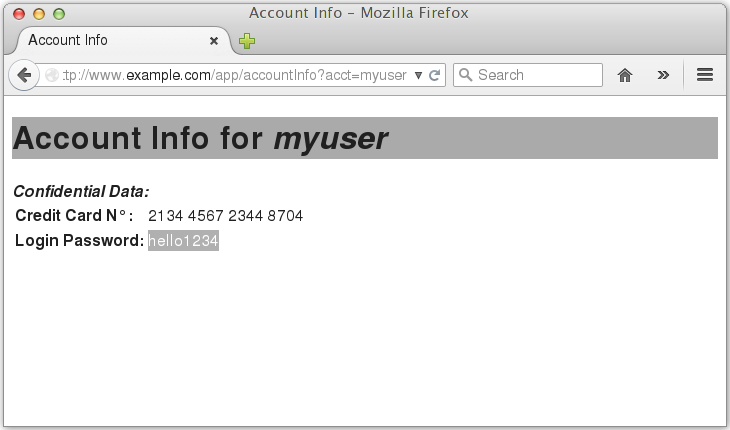
\includegraphics[width=4cm]{example_web_s1}\\
   \LARGE{Attack behavior}\\\normalsize Example URL: \small\texttt{http://somesite.net/change password?user=\textit{otheruser}}\\
   \normalsize{Result:}\\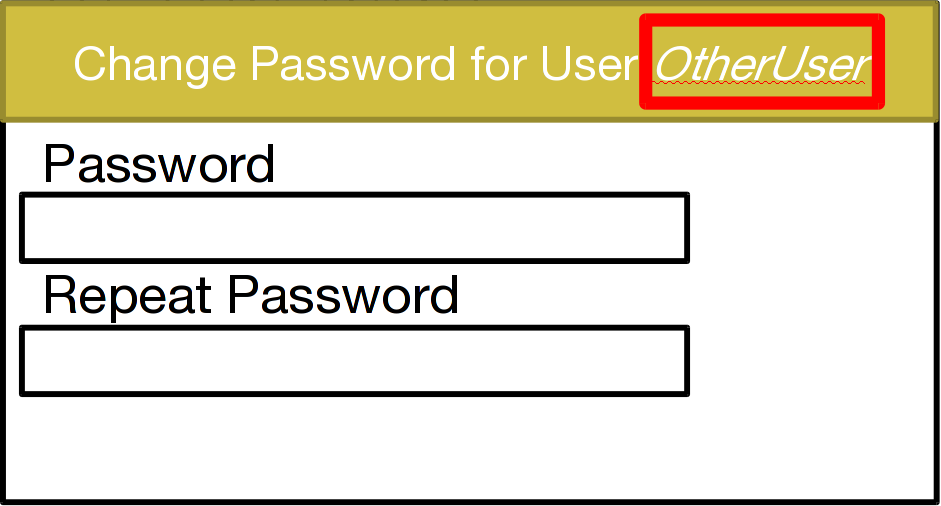
\includegraphics[width=4cm]{example_web_s2}\\
  \end{multicols}
\end{frame}

\begin{frame}
  \frametitle{Example: Attack}
  This URL:\\ \texttt{/changepassword?user=\textit{otheruser'; DROP tbl\_user; }} (\ref{examplecode})
\end{frame}


\section{How to prevent an Attack}

\begin{frame}
  \frametitle{Solutions and Problems}
\tiny
  \begin{tabular}{|l|p{4cm}|p{4cm}|}
    \hline
    & \textbf{Advantage} & \textbf{Disadvantage} \\\hline
    \textbf{Session Based} & Only one authorization has to be done, access data for Database etc. is saved on the server and is not accessible by the attacker & A session uses a lot of memory for each user. For applications with a high number of users, a session for each client is not possible i.e. a non-session solution has to be implemented \\\hline
    \textbf{Authorization} & TBD & TBD\\\hline
  \end{tabular}
\end{frame}

\end{document}